% \title{Measurement: Errors and Error Analysis}
% \author{An Introduction to Physics through Experiments}
% \date{}
% \maketitle

\chapter{Measurement: Errors and Error Analysis}
\section{Objectives}

\begin{enumerate}
    \item To learn to use the Vernier Calliper and Screw Gauge.
    \item To study the propagation of errors from measured to derived quantities.
\end{enumerate}


\section{Theory: Measurement}

\subsection{The Vernier Calliper}

You will regularly come across vernier scales in the lab when using callipers, screw-gauges, angular vernier scales (in spectrometers), and travelling microscopes. Vernier scales allow you to read off a value more precisely than when using an ordinary scale. In this section, we will explain how this works.

First consider a `main scale' with a least count of 1 unit (you could imagine this is $1mm$, if you wish). This implies that any distance between, say, the 2 and 3 unit marks cannot be determined accurately. In other words, the best you could say is that an object is ``2 and a bit'' units. The vernier scale allows you to \textbf{quantify} this `bit'.  

The method is rather ingenious: the vernier scale has a certain number of divisions (say 10, for the purpose of our example) that are equally spaced (see Figure (\ref{fig:vernier_1})). These 10 divisions are set to coincide with 9 divisions of the main scale.

\begin{question}
    \paragraph{Question:} What is the spacing between two vernier scale divisions? Is it:
    \begin{enumerate}
        \item 1 unit?
        \item 0.1 units?
        \item 0.9 units?
    \end{enumerate}
\end{question}



\begin{figure}[!htb]
    \centering
    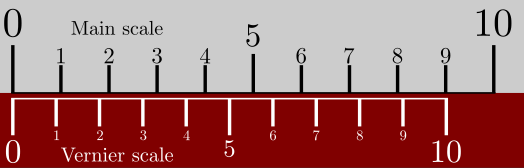
\includegraphics[scale=0.75]{figs/vernier1.png}
    \caption{10 vernier scale divisions are set to coincide with 9 main scale divisions.}
    \label{fig:vernier_1}
\end{figure}

Let us now try to measure the smallest possible distance between 0 and 1 unit. Take a Vernier Calliper and close it completely. If there is no zero-error, the only two readings on the vernier scale and main scale that match are the $0$ and $10$ divisions.

\begin{figure}[!htb]
        \begin{subfigure}[b]{0.5\textwidth}
                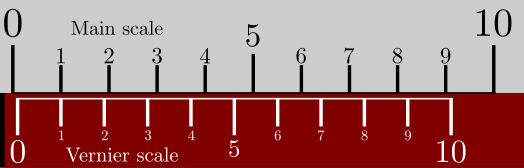
\includegraphics[width=0.95\linewidth]{figs/vernier2.png}
                \caption{Just away from 0, when the coinciding division \\is 1, the distance is $1\times\texttt{MSD}-1\times\texttt{VSD}=0.1\, \texttt{units}$.}
                \label{fig:vernier_2}
        \end{subfigure}\hfill
        \begin{subfigure}[b]{0.5\textwidth}
                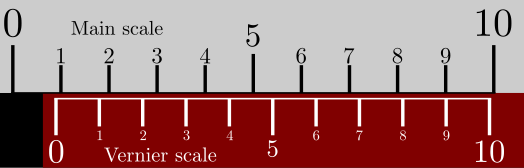
\includegraphics[width=0.95\linewidth]{figs/vernier3.png}
                \caption{Before crossing 1, the last coinciding division is 9, and the distance is $9\times\texttt{MSD}-9\times\texttt{VSD}=0.9\, \texttt{units}$.}
                \label{fig:vernier_3}
        \end{subfigure}%
        \caption{Measurement with a Vernier Calliper.}
        \label{fig:verniermeasurements}
\end{figure}

\begin{enumerate}
    \item Move the vernier scale \textit{slightly}, until the $1$ on the vernier scale coincides with the nearest main scale division (this is obviously the $1$ on the main scale, see Figure (\ref{fig:vernier_2})).
    
    \item You will notice that the jaws are slightly apart. The distance between them is of course the distance the $0$ on the vernier scale has moved.
    
    \item But this distance is simply the difference between 1 Main Scale Division (\texttt{MSD}) and 1 Vernier Scale Division (\texttt{VSD}), since both the $1s$ coincide!
    
    \item Thus, the spacing between the jaws of the calliper is now $0.1$ units!
    
    \item We have thus been able to measure a distance of $0.1$ units using two scales, one of least count $1$ unit, and the other of least count $0.9$ units!
\end{enumerate}

Similarly, if you went one division further, and had the 2 of the vernier scale coincide with a main scale division, then the distance between the jaws would be $2\times\texttt{MSD}-2\times\texttt{VSD}=0.2\, \texttt{units}$. Thus, if the $n$th vernier scale division coincides with a main scale division, the distance between the jaws is $n \times (\texttt{MSD}-\texttt{VSD})=n \times \texttt{LC}$. Where \texttt{LC} is the Least Count of the Vernier Calliper\footnote{In our case, the Least Count is 0.1 units.}.

Of course, up until right now we have been measuring distances between 0 and 1 unit.  What about an arbitrary distance? Consider the example given in Figure (\ref{fig:vernier_4}). 

\begin{figure}[!htb]
    \centering
    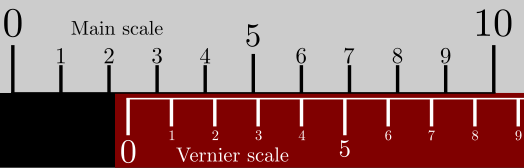
\includegraphics[scale=0.75]{figs/vernier4.png}
    \caption{The main scale reading is more than 2 units. The coinciding vernier scale division is 4 . }
    \label{fig:vernier_4}
\end{figure}

Here is the general procedure to take a reading using a vernier calliper,

\begin{enumerate}
    \item Look where the zero mark on the vernier scale meets the main scale. This gives us our rough reading, usually called the Main Scale Reading or \texttt{MSR}. In the example in Figure (\ref{fig:vernier_4}), the \texttt{MSR} is 2.
    
    \item Now look to find the mark on the vernier scale which most closely meets any mark on the main scale. This is the Vernier Scale Reading or \texttt{VSR}, giving you the most precise digit. In this example, the \texttt{VSR} is 4.
    
    \item The total distance is given by 
    $$\texttt{distance} = \texttt{MSR} + \left(\texttt{VSR}\times\texttt{LC}\right)$$
    
    In our case, $\texttt{distance} = 0.24$ units.
    
    \item Thus, using two scales -- one of least counts $1$ unit and another of least count $0.9$ units -- we have a calliper capable of measuring upto $0.1$ units!
\end{enumerate}

\begin{question}
\paragraph{Question:} Show that the least count of a Vernier Calliper is given by:
\begin{enumerate}
    \item $$\texttt{LC} = \texttt{Least count of main scale} - \texttt{Least count of vernier scale}$$
    \item $$\texttt{LC} = \frac{\texttt{Least count of main scale}}{\texttt{Number of vernier scale divisions}}$$
\end{enumerate}
\end{question}

\subsection{The Micrometer Screw Gauge}

The micrometer screw gauge was invented in the 17th century as an enhancement of the vernier callipers, and is used to measure even smaller dimensions. The screw gauge uses a screw with an accurate amd constant \textbf{pitch} (the amount by which the thimble moves forward or backward for one complete revolution) as an auxiliary scale marked on a rotatable thimble.  

The micrometers in our laboratory have a pitch of 0.01$mm$.  The rotating thimble is subdivided into 100 equal divisions.  The thimble passes through a frame that carries a millimetre scale graduated to 1$mm$.  The jaws can be adjusted by rotating the thimble using the small ratchet knob.  This includes a friction clutch which prevents too much tension from being applied.

\begin{imp}
Only tighten the screw gauge by rotating the ratchet, otherwise you may damage the instrument. Stop rotating after you hear \textbf{three} clicks. \textbf{Do not} tighten the screw any further.
\end{imp}

\begin{question}
\paragraph{Question:} Show that the least count of a screw gauge is given by
$$\texttt{LC} = \frac{\texttt{Pitch of a the screw}}{\texttt{Number of circular scale divisions}}$$
\end{question}

We won't go into using a screw gauge in much more detail as its function very similar to the Vernier Calliper, except with a finer least count.

\section{Theory: Error Analysis}

\subsection{Types of Errors}

``Error'' analysis is a rather glaring misnomer. All measurements have some degree of uncertainty that may come from a variety of sources, from the lack of precision of the measuring instrument to random fluctuations in the environment. The process of evaluating the uncertainty associated with a measurement result is often called uncertainty analysis or error analysis. However, the common definition of an ``error'' being a ``mistake'' is very misleading. However, the terminology is so rampant that we will be forced to use it at times, referring to `error' analysis when we really mean `uncertainty' analysis.


\begin{tip}
Example: if you use a metre scale with a least count (smallest division) of $0.1cm$ upside down to measure a pencil and misread the scale as $94.6cm$ instead of $5.4cm$, this is a \textbf{mistake}.\\

However, if you note down the length as being $5.4cm$, but rightly note that it is not \textbf{exactly} $5.4cm$, but simply that your measuring device does not allow for any more precision, this is a measure of \textbf{uncertainty}. \\

We will expect you to have verified that you haven't done the former, and will take for granted from here on that no mistakes were made in the collection of data.
\end{tip}


The complete statement of a measured value \textbf{must} include an estimate of the level of confidence associated with the value. This allows people to judge the quality of the experiment and allows for comparisons with other similar estimates of the same quantity, or theoretical prediction.  

\begin{imp}
A proper experiment must report both a `best' value and an uncertainty for each measured quantity. You will be expected to do this in all your experiments. 
\end{imp}

Without an uncertainty estimate, it is impossible to answer the basic scientific question: ``Does my result agree with a theoretical prediction or results from other experiments?'' This question is fundamental for deciding if a scientific hypothesis is confirmed or refuted.

\begin{tip}
\paragraph{A cautionary tale:} Neutrinos are weakly interacting nearly massless particles that are theorised to be moving close to -- if not at -- the speed of light.\\

In September 2011, scientists of the OPERA collaboration reported evidence that neutrinos they produced at CERN in Geneva and recorded at the OPERA detector at Gran Sasso, Italy, had travelled \textbf{faster} than light. If this were true, it would have violated one of the pillars of modern physics, the Theory of Relativity.\\

The neutrinos were calculated to have arrived approximately 60.7 nanoseconds sooner than light would have if it had traversed the same distance in a vacuum. Assuming the error were entirely due to random effects, scientists calculated that there was a 0.2-in-a-million chance that this may be a false positive.\\

In March 2012 it was confirmed that a fibre cable was not fully screwed in during data gathering, and this effectively decreased the reported flight time of the neutrinos by 73ns, making them seem faster than light. The corrected difference between the measured and expected arrival time of neutrinos (compared to the speed of light) was approximately 6.5 $\pm$ 15 ns. This is consistent with \textbf{no difference at all}, thus the speed of neutrinos is consistent with the speed of light within the margin of error.
\end{tip}

\subsubsection{Least count errors}

As you have already seen, the least count of a measuring instrument is the smallest value the instrument can resolve. For example, if we use a metre scale to measure an object and find that it is $23.5$cm, the uncertainty here \textbf{due to the measuring instrument} is $0.1$cm. Thus, we can say that the length of the object is given by $l = (23.5 \pm 0.1) cm$ where $\pm \Delta l = \pm 0.1$cm is the uncertainty in measurement due to the least count of the metre scale. This is the value up to which the `best' value of $23.5$ may be specified with any confidence.

In general, such errors are the \textbf{lower bounds} of experimental errors. No error that is less than the least count error need be considered. That being said, if you find other sources of error to be greater than the least count error, then those sources should be used. For example, the stopwatches in the lab have a least count of $0.01$s. However, your reaction time of turning on and off a stopwatch would be at best $0.1$s. Thus, while the least count error is significantly smaller, the \textbf{actual} error in a time measurement using the stopwatch would be of the order of $0.1$s.

\subsubsection{Systematic errors}

Imagine now that the metre scale that you are using to measure the length of the object is made of metal, and as a result expands slightly in summer. If you performed a set of measurements, you would obviously not find the `true' value of the length. However, such an error may be discovered by comparing your measurements from the metal scale with a wooden scale, for example. When using instruments like digital multimeters you obviously rely on it having been calibrated properly. However, there might have been an accident that a student did not report, and as a result there could well be a systematic error for someone unlucky enough to be the one using it next.

Estimating possible errors due to such systematic effects depends on your understanding of your apparatus and the skill you have developed for thinking about possible problems. In this course for the most part such errors will be assumed to be small. However, if you get a value for some quantity that seems rather far off what you expect, you should think about such possible sources more carefully. You could end up trusting a device that you do not know is faulty. This happens very often, to the best of us. 


\subsubsection{Random errors}

Another reason for two measurements not agreeing totally is due to small, uncorrelated variations in the environment or measurement process. For example, while measuring the time period of a pendulum, you might get different readings due to small differences in your reaction time. Similarly, when measuring the height of a cylinder with a vernier calliper, you may see small variations depending on \textbf{where} you measure the height, as it is possible the cylinder was not made to be smooth up to $0.1$mm everywhere.

Such variations, being \textbf{random}, are expected to fall just as often \textit{above} a certain value as \textit{below} it. A truly random source would give you a \textbf{Gaussian} distribution of errors; the mean of this distribution $$\overline{m}_N = \frac{\sum_{i=1}^{N}{m_i}}{N}$$ would approach the `best' value as the number $N$ of well-sampled values increases. The uncertainty of these measurements would then be quantified by the \textbf{standard deviation}\footnote{There is a reason for the $N-1$, it is known as the number of `degrees of freedom' in statistics. Understanding it is not essential for this course.} $$\Delta m_N = \sqrt{\frac{(m_i - \overline{m}_N)^2}{N-1}}$$

more conventionally denoted by $\sigma$.


\subsubsection{Precision, Accuracy, and Statistics}

\begin{enumerate}
    \item \textbf{Accuracy:} is how closely a measurement comes to some `true' value. It determines how well we have eliminated \textbf{\textit{systematic errors}} and mistakes in our measurements.
    \item \textbf{Precision:} is how closely a set of measurements agree \textit{with each other}. It determines how well we have eliminated \textbf{\textit{random errors}} in our measurements.
\end{enumerate}

To use a sports simile, if you're playing football and are accurate, your aim will always take the ball close to or into the goal. If, however, you harbour a personal grudge against the coach and succeed in beaning him on the head every time you get the ball, then you would be \textit{precise}, but not accurate\footnote{It is widely accepted that the point of football get the ball into the goal and not to traumatise your coach, which is why this example works.}.

\textbf{A caveat:} In any Physics experiment worth doing, you usually don't have the answer beforehand. This means you don't have a `true' value with which to compare your answer. This is why it is so important to be both precise (reduce all random errors present in your measurements) and accurate (reduce all systematic errors present in your measurement). You must also, however, come up with ways to check if your answer is accurate \textit{without} trying to resort to a `textbook' solution.

\begin{question}
\paragraph{Question:} In the example of the `superluminal' neutrinos given earlier, was the error of the OPERA team one of inaccuracy, or of imprecision? 
\end{question}

\textbf{A note on statistics:} Consider two sets of measurements of the acceleration due to gravity:

\begin{table}[!htb]
\parbox{.45\linewidth}{
\centering
\begin{tabular}{cc}
\hline
\textbf{S. No.}&$\bm{g}\,\, (ms^{-2})$\\
\hline
1&$9.80\pm0.01$\\
2&$0.70\pm0.01$\\
3&$18.90\pm0.01$\\
4&$15.60\pm0.01$\\
5&$4.10\pm0.01$\\
\hline
Mean&$9.82\pm0.01$\\
\hline
\end{tabular}
\caption{Measurement of $g$ (Set 1)}
}
\hfill
\parbox{.45\linewidth}{
\centering
\begin{tabular}{cc}
\hline
\textbf{S. No.}&$\bm{g}\,\, (ms^{-2})$\\
\hline
1&$9.83\pm0.01$\\
2&$9.80\pm0.01$\\
3&$9.82\pm0.01$\\
4&$9.84\pm0.01$\\
5&$9.83\pm0.01$\\
\hline
Mean&$9.82\pm0.01$\\
\hline
\end{tabular}
\caption{Measurement of $g$ (Set 2)}
}
\end{table}

It would obviously be wrong to go simply by the mean and say that both these sets of data were equally reliable. In fact, stating the mean of the first set as the acceleration due to gravity \textbf{doesn't make sense}. 

Suppose we compared the mean of a data set to its \textit{dispersion} about the mean. If this is small, we could then say that there is some `true' value and that all the different values we measured occurred due to random fluctuations about this `true' value. Since the fluctuations are random, we could assume that they average out to zero, leaving us with a closer estimate to the `true' value than any individual reading.

When the significant source of error is considered to be random, the distribution is a Gaussian, and the measure of dispersion is the \textbf{standard deviation} denoted by $\sigma$. \textit{In such a case}, the error $\delta x$ in the reading could be taken to be $\sigma_x$ without much loss of generality, as it can be shown that there is a 68\% likelihood that an individual measurement will fall within one standard deviation $(\pm\sigma_x)$ of the true value\footnote{Keep in mind, however, the example of superluminal neutrinos we gave earlier: in that case, the error was \textit{assumed} to be random, and their precise data led them to a false positive. The true error turned out to be systematic, leading to \textit{different (and larger) error bars}!}. 

\begin{question}
\paragraph{Question:} In above sets of data (with standard deviations of $7.6\,\,ms^{-2}$ and $0.02\,\,ms^{-2}$ respectively), does the quoted error of $\pm 0.01\,\, ms^{-2}$ make sense
\begin{enumerate}
    \item For Set 1?
    \item For Set 2?
    \item For Both?
    \item For Neither?
\end{enumerate}
Justify your answer quantitatively.
\end{question}

\begin{imp}
The two errors in the lab you will encounter that you cannot remove are \textbf{least count errors} and \textbf{random errors}. Remember to always compare them and \textbf{\textit{take the larger value}}. In Set 1 it makes no sense to say $g$ is specified to $(9.82\pm0.01)\,ms^{-2}$, since all of the values are much farther away than that!
\end{imp}

\begin{question}
\begin{enumerate}
    \item \textbf{Question:} Multiple measurements with the same instrument increases the
    \begin{enumerate}
        \item Accuracy
        \item Precision
        \item Both
    \end{enumerate}
    
    \item \textbf{Question:} Consider the following data-table~\\
    \begin{tabular}{cccccc}
    \hline
    \textbf{S. No.}&1&2&3&4&5\\
    \hline
    \textbf{Time Period} ($s$)& $1.2\pm0.1$&$1.2\pm0.1$&$1.2\pm0.1$&$1.2\pm0.1$&$1.2\pm0.1$\\
    \hline
    \end{tabular}~\\~\\
    The standard deviation is $0.0$. Would it be right to say that $T_\text{avg} = 1.2\pm 0.0$?
\end{enumerate}
\end{question}

However, keep in mind there are many cases where the mean  \textbf{does not} represent some true value\footnote{For example, even if the average number of siblings every student has is $1.574$, there is no student who has a non-integer number of siblings.}. There are also cases where the standard deviation contains physical information. Such cases are usually a result of statistical phenomena.

\begin{tip}
\begin{enumerate}
    \item In a coin-toss experiment with a large number of tosses, $\sigma$ gives you a measure of the bias of the coin.
    \item In a random walk, $\sigma$ can be a measure of the diffusion coefficient $D$.
    \item In shot-noise --  the statistical fluctuations of current due to the actual number of electrons flowing in the conductor per unit time -- $\sigma$ gives you a measure of Boltzmann's constant $k_B$.
\end{enumerate}
\end{tip}


\subsection{Reporting Errors}
\subsubsection{Significant figures}

The significant figures of a number are the digits in its representation that contribute to the precision of the number. In practice, we assume that all digits used to write a number are significant (except leading zeroes\footnote{Non-leading zeros are considered to be significant. If you write a number as 1,200, we assume there are four significant digits. If you only mean to have two or three, then it is best to use scientific notation: $1.2 \times 10^3$ or $1.20 \times 10^3$ . Leading zeros are not considered significant: 0.55 and 0.023 have just two significant figures.}).

\textbf{Results of simple calculations should not increase the number of significant digits}. Calculations transform our knowledge; they do not increase it! The rounding should be performed at the final step of a calculation to prevent rounding errors at intermediate steps from propagating through your work but \textbf{only} one or two
extra digits suffice to prevent this.

If you measure a value on a two-digit digital meter to be 1.0 and another value to be 3.0, it is incorrect to say that the ratio of these measurements is 0.3333333. The two values are not exact numbers with infinite precision. Since they each have two significant digits, the correct number to write down is 0.33\footnote{If this is an intermediate result, then 0.333 or 0.3333 are preferred, but the final result must have two significant digits.}.

\begin{imp}
\textbf{Do not write significant figures beyond the first digit of the error on the quantity}. Giving more precision than this to a value is not only irrelevant, \textit{it is misleading}.\\

If you're told you're using FAR too many digits, please do not try to use the excuse, ``That's what the computer gave me.'' \textbf{You} are in charge of presenting your results, not the computer!
\end{imp}


\subsubsection{Error propagation}

Experiments worth carrying out rarely measure only one quantity. Typically we measure two or more quantities and then `fold' them together in some equation or equations to determine some other quantity that we believe to depend on them. It is thus imperative that we understand how uncertainties in certain measured quantities `propagate' into other derived quantities.

For our analysis, let us assume that

\begin{itemize}
    \item $x$ and $y$ are measured quantities with uncertainties $\delta x$ and $\delta y$ respectively. These errors are considered to be \textbf{uncorrelated}, meaning that $\delta x$ and $\delta y$ are independent\footnote{For example, the precision of measuring the length of your simple pendulum has no effect on the precision of measuring time.}.
    
    \item $c$ is a constant known to known absolutely precisely (or with negligible uncertainty).
    
    \item $z$ is a quantity \textit{derived} from $x$ and $y$ and possessing a `propagated' uncertainty $\delta z$.
\end{itemize}

The formulae used to compute errors are usually not completely understood: a variety of different formulae are used in different cases, and the reasons \textbf{why} are usually lost on students. It turns out that there is only \textbf{one} way to add (uncorrelated) errors, which one can manipulate to get the rest:

\begin{imp}
If $z = x + y$, their (uncorrelated) errors add \textbf{in quadrature}:
\begin{equation}
    \delta z = \sqrt{\left(\delta x\right)^2+\left(\delta y\right)^2}
    \label{quadrature}
\end{equation}
\end{imp}

The reason for errors adding in quadrature is one that comes from statistics; it is essential that the errors be \textbf{independent} of each other (uncorrelated)\footnote{It also makes sense:  errors could be positive and some negative, simply adding them could conceivably give a smaller number (or even zero!). Thus, the next best thing is to add their \textit{squares}. }

Here is another motivation\footnote{This is \textbf{not} an explanation of why this is true!}: you could imagine two uncorrelated measurements to represent two axes ($x$ and $y$) that are orthogonal to each other (see Figure (\ref{fig:quadrature}). Imagine that you want to specify a point $z = (x,y)$: given that there is an uncertainty in both the coordinates $x$ and $y$, the point $z$ is uncertain \textbf{at most} by $\delta z = \sqrt{\left(\delta x\right)^2+\left(\delta y\right)^2}$.

\begin{figure}
    \centering
    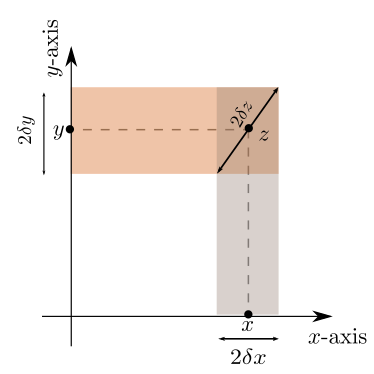
\includegraphics[scale=0.5]{figs/quadrature.png}
    \caption{Two points $(x,0)$ and $(0,y)$, with uncertainties $\delta x$ and $\delta y$ respectively, can be summed to get a point $z=(x,y)$ with uncertainty $\delta z$. }
    \label{fig:quadrature}
\end{figure}

This formula can then be used to get the uncertainties of more complicated relations. For example, consider $z = xy$. In this case, the two quantities are \textbf{multiplied}, and so we can't use the above formula as is. We could, however, take the log, and get $\log{z} = \log{x} + \log{y}$. This is of the form $u = v + w$. We could then apply Equation (\ref{quadrature}), and find that $$\delta \left(\log{z}\right) = \sqrt{\left(\delta \left(\log{x}\right)\right)^2 + \left(\delta \left(\log{y}\right)\right)^2}$$

The uncertainty in $\log{z}$ can easily be related by taking the derivative\footnote{A differential is by definition the variation of function when its parameter changes by a small amount. We want to find how much $\log{z}$ changes when $z$ changes by $\delta z$. We use $\delta$ instead of $\dd$, since the variation is not truly \textit{infinitesimal}.}.

\begin{equation*}
    \dd({\log{z}}) = \frac{\dd z}{z} \quad \implies \quad \delta (\log{z}) = \frac{\delta z}{z}
\end{equation*}

Thus, 

\begin{equation}
    \frac{\delta z}{z} = \sqrt{\left(\frac{\delta x}{x}\right)^2 + \left(\frac{\delta y}{y}\right)^2}
\end{equation}

\begin{tip}
The following rules should exhaust most of the common cases that you will be exposed to in your undergraduate labs. Everything here can be generalised simply to a a \textit{set} of measurements $x_i$ with uncertainties $\delta x_i$.

\begin{enumerate}
    \item \textbf{Addition or subtraction by a constant:} If $z = c \pm x$, then 
    \begin{equation}
        \delta z = \delta x
    \end{equation}
    
    
    \item \textbf{Multiplication by a constant:} If $z = c x$, then 
    \begin{equation}
        \delta z = c\delta x
    \end{equation}
    
    \item \textbf{Addition or subtraction of two measured quantities:} If $z = x \pm y$, then 
    
    \begin{equation}
        \delta z = \sqrt{(\delta x)^2 +(\delta y)^2}
    \end{equation}
    
    \item \textbf{Multiplication or division of two measured quantities:} If $z = xy$ or $z = \frac{x}{y}$, then 
    
    \begin{equation}
        \frac{\delta z}{z} = \sqrt{\left(\frac{\delta x}{x}\right)^2 + \left(\frac{\delta y}{y} \right)^2}
        \label{relerror}
    \end{equation}
    
    \item \textbf{A measured quantity raised to a power:} If $z = x^c$, then
    
    \begin{equation}
        \frac{\delta z}{z} = c \frac{\delta x}{x}
        \label{powerror}
    \end{equation}
    
\end{enumerate}
\end{tip}

\begin{question}
\paragraph{Question:} Prove Equation (\ref{powerror}).~\\

\paragraph{Question:} If $z = x^2 = x \times x$, we get different answers if we use the Power Rule (Equation (\ref{powerror})) or the Product Rule (Equation (\ref{relerror})). Which of the two is correct? Why? ~\\

\paragraph{Question:} Calculate the uncertainty in $z$ if
\begin{enumerate}
    \item $z = \frac{1}{x}$
    \item $z = \frac{x}{1+x}$
    \item $z = \frac{x}{x+y}$
\end{enumerate}
\paragraph{Hint:} The last one is slightly hard. You will first write it as $z = \frac{1}{1 + u}$, where $u = y/x$. Then, calculate $\delta z$ in terms of $\delta u$, and only then $\delta u$ in terms of $\delta x$ and $\delta y$.
\end{question}

\section{Apparatus}

\begin{enumerate}
    \item A pair of Vernier Callipers
    \item A Screw Gauge
    \item A set of ball bearings
    \item A set of aluminium cylinders
    \item A conical measuring flask
    \item A container with a spout
\end{enumerate}

\section{Description}

\begin{enumerate}
    \item In \textbf{Part A} you will measure the radius, height, and volume of different cylinders. You will then plot an appropriate graph from which you will extract the value of $\pi$.
    
    \item In \textbf{Part B} you will measure the radius and volume of different ball bearings. You will then plot an appropriate graph from which you will extract the value of $\pi$.
    
\end{enumerate}

\section{Suggested Procedure}

\subsection{Part A}

\begin{enumerate}
    \item Decide on the best instrument and method to measure the following properties of the cylinders:
    \begin{enumerate}
        \item Radius
        \item Height
        \item Volume
    \end{enumerate}
    
    \begin{question}
        \paragraph{Question:} How and where would you measure the radius of the cylinders? How many trials would you take?
    \end{question}
    
    \item Be sure to take a sufficient number of \textbf{well-sampled} readings.
    
    \item Decide on an appropriate graph between the measured quantities from which you can extract the numerical value of $\pi$.
\end{enumerate}

\subsection{Part B}

\begin{enumerate}
    \item Decide on the best instrument and method to measure the radii and the volumes of the bearings.
    
    \item Be sure to take a sufficient number of \textbf{well-sampled} readings.
    
    \item Decide on an appropriate graph between the measured quantities to extract the numerical value of $\pi$.
\end{enumerate}

\begin{question}
\paragraph{Question:} How does your estimate compare with the known value of $\pi \approx 3.14159$?
\end{question}



\newpage